\documentclass{beamer}

\usetheme{Rochester}
\usecolortheme{material}
\usepackage{multicol}
\usepackage{listings}

\setbeamertemplate{footline}[text line]{%
  \parbox{0.5\linewidth}{
    \vspace*{-12pt} %\insertshorttitle~(\insertshortauthor)
  }
  \hfill%
  \parbox{0.5\linewidth}{
    \vspace*{-12pt}\raggedleft\insertpagenumber
  }
}
\lstset{
breaklines=true, 
basicstyle=\scriptsize, 
keywordstyle=\color{blue700},
basewidth=0.55em
}
\setbeamertemplate{navigation symbols}{}
\begin{document}
\title[Entwurssprachen]{HW/SW Codesign LU - FLAC Decoder}
\author[Platzer M., Zaruba F., Weber T.]{Michael Platzer, Florian Zaruba, Thomas Weber}
\date{\today}

\begin{frame}
\titlepage
\end{frame}

\begin{frame}\frametitle{Table of contents}
%\begin{multicols}{2}
  \tableofcontents
%\end{multicols}
\end{frame}

\section{Partitioning} 
\begin{frame}\frametitle{Partitioning} 
Ideas for the Implementation
\begin{itemize}
	\item SD-Card read in HW
	\item Display and FFT in HW
	\item ... TBA
	\item Optimizations in C code (loop unrolling,..)
\end{itemize}
\end{frame}

\section{SDCard}
\begin{frame}\frametitle{SDCard}
	
\end{frame}
\begin{frame}\frametitle{RA - Overview}
    \begin{figure}[hp]
      \centering
      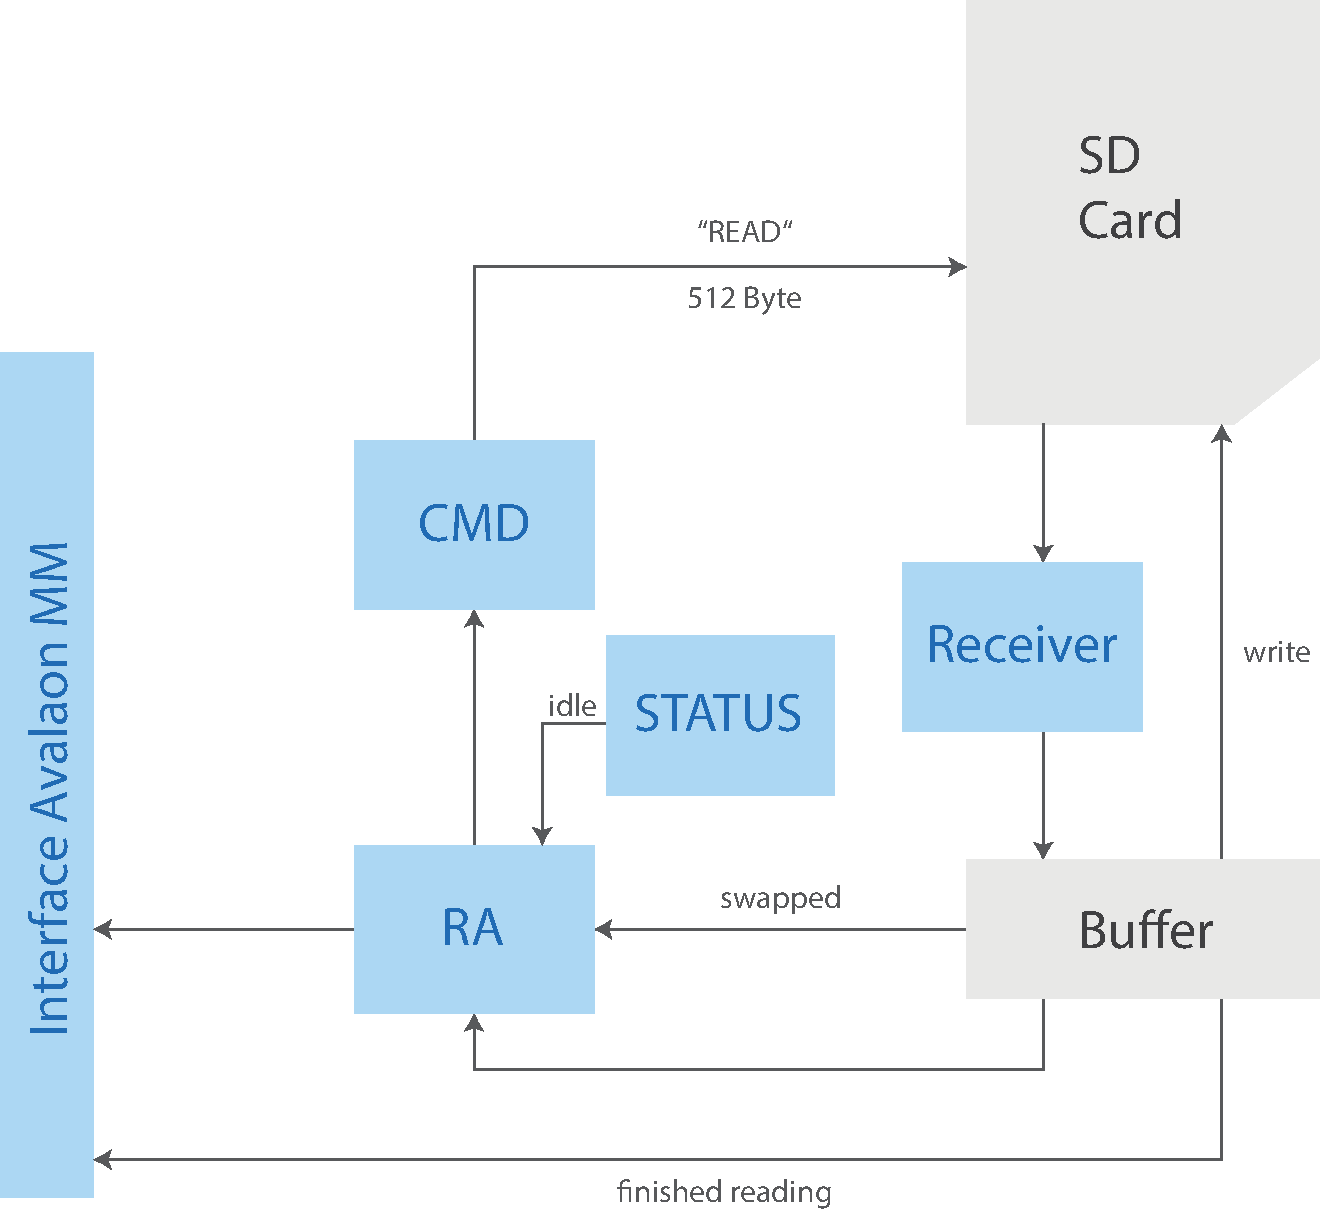
\includegraphics[width=0.6\textwidth]{pictures/read_ahead_overview}
      \caption{Read-ahead overview}
      \label{fig:fft_display_struct}
    \end{figure}
\end{frame}

\begin{frame}\frametitle{RA - Buffer}
    \begin{figure}[hp]
      \centering
      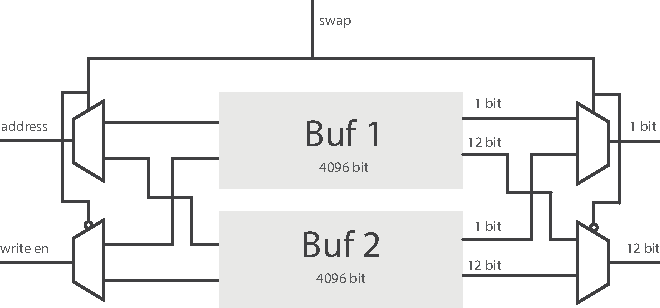
\includegraphics[width=0.7\textwidth]{pictures/read_ahead_gatter}
      \caption{Read-ahead RTL}
      \label{fig:fft_display_struct}
    \end{figure}
\end{frame}

\section{FFT - Display}
\begin{frame}\frametitle{FFT-Display}
    \begin{figure}[hp]
      \centering
      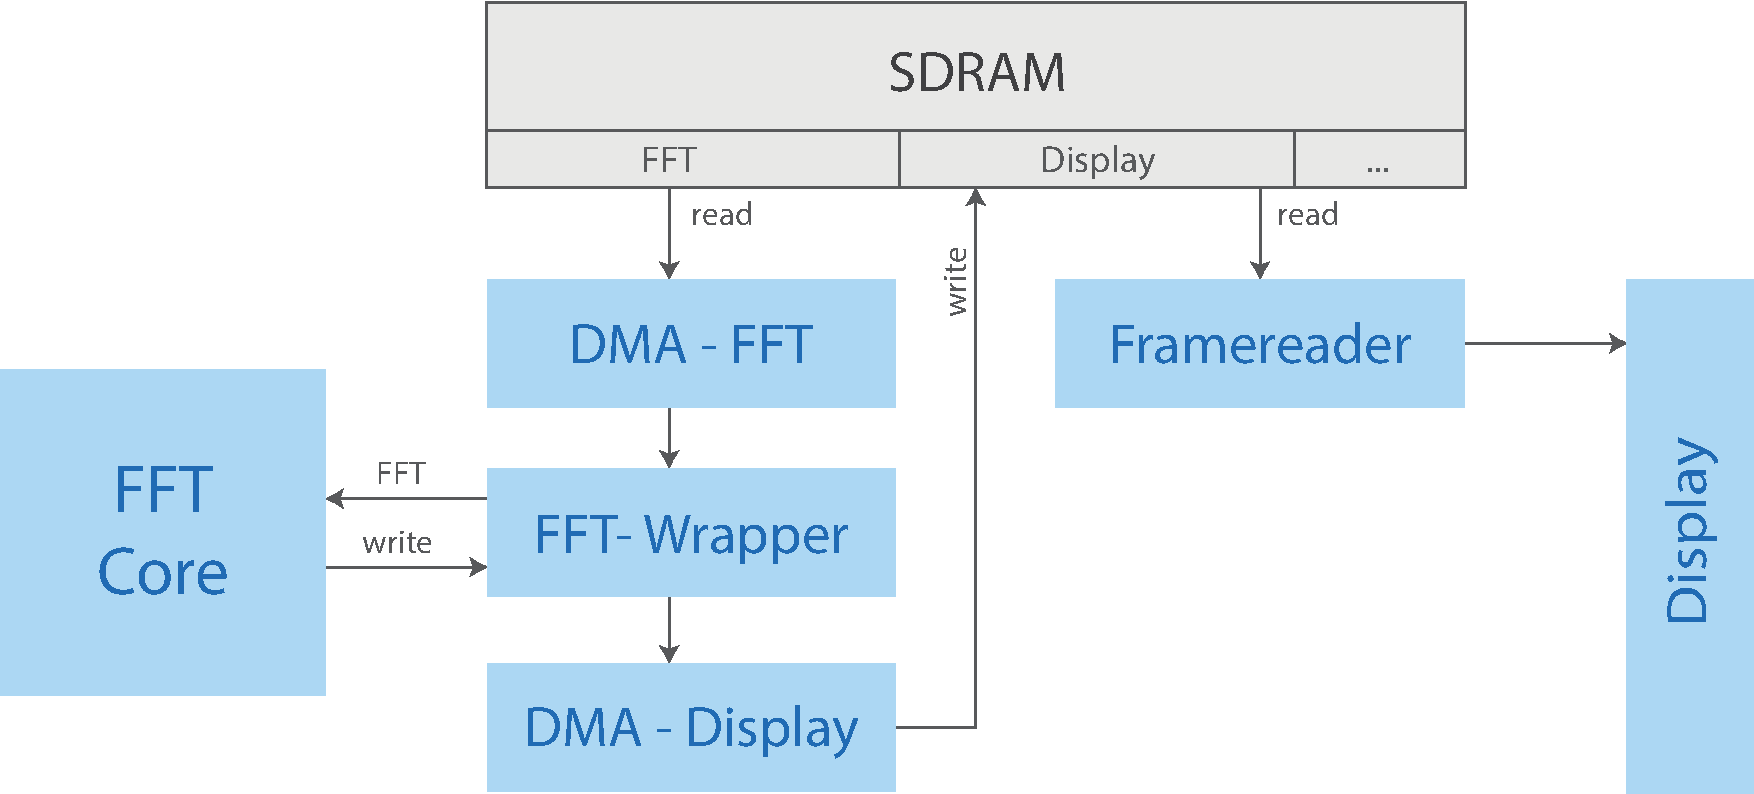
\includegraphics[width=0.9\textwidth]{pictures/fft_display}
      \caption{FFT Display overview}
      \label{fig:fft_display_struct}
    \end{figure}
\end{frame}
\section{Software}
\begin{frame}[fragile]\frametitle{Software - Bit Reader}
    Bit Reader
    \begin{itemize}
    \item 512 bytes (4096 bits) read at once from SD card
    \item Stored in buffer with bytes of each 32 bit word inverted
    \item Bit reader context provides functions to read bits, which must
    not be aligned and can overlap words and blocks
    \item Functions match requirements to decode FLAC frames
    \end{itemize}
    \begin{lstlisting}[language=C]
    int get_bits(int n);     // read up to 32 bits
    int get_unary1(int max); // read unary encoded value
    ...
    \end{lstlisting}
\end{frame}
\begin{frame}[fragile]\frametitle{Software - Get Bits}
    \begin{lstlisting}[language=C]
uint32_t buf[128]; // 512 byte = 4096 bit buffer
int pos;           // bit position in buf

unsigned int get_bits(int n)
{
    if (pos >= 4096)
        read_block(); // read next sd card block into buf

    // read first word into cache:
    uint64_t cache = (uint64_t)buf[pos >> 5] << 32;

    // if bits to be read overlap two words, read next word:
    if ((pos & 0x1f) + n > 32)
        cache |= (uint64_t)buf[(pos >> 5) + 1];

    // shift out bits which must not be returned:
    uint64_t ret = (cache << (pos & 0x1f)) >> (64 - n);
    pos += n;
    return ret;
}
    \end{lstlisting}
\end{frame}
\begin{frame}[fragile]\frametitle{Software - LPC decoding}
    Decode LPC coded samples:\\
    $s_i$ : sample, $r_i$ : residual, $c_i$ : LPC coefficient, $p$ : predictor order
    $$ s_n = r_n + \prod_{i=0}^p s_{n-i} \cdot c_i $$
    Naive code with nested loops:
    \begin{lstlisting}[language=C]
    for (i = pred_order; i < len; i++, decoded++) {
        int sum = 0;
        for (j = 0; j < pred_order; j++)
            sum += coeffs[j] * decoded[j];

        decoded[pred_order] += sum >> shift;
    }
    \end{lstlisting}
    Optimize to reduce branches and memory accesses
\end{frame}

\section{Problems}
\begin{frame}\frametitle{Problems}
\begin{itemize}
	\item {TBA} 
	\item {TBA}
	\item {TBA}
	\item {TBA}
\end{itemize}
\end{frame}
      
\section{Bibliography}
%\nocite{haubelt2010digitale}
%\nocite{canis2011legup}
%\nocite{liao2002system}
%\nocite{initiative2014functional}
\begin{frame}[allowframebreaks] \frametitle{Literature} 
\bibliographystyle{plain}
\bibliography{references}
\end{frame}



\end{document}
